\documentclass[a4paper,11pt]{report}
\usepackage[utf8]{inputenc} % un package
\usepackage[francais]{babel} %active le mode francais
\usepackage[top=2cm , bottom=2cm , left=2cm , right=2cm]{geometry} %propriétés de notre page
\usepackage{amsmath} %liste de symboles et applications mathématiques
\usepackage{amsfonts} %idem
\usepackage{color} %Permet d'utiliser la couleur dans nos documents
\usepackage{listings} %Paquet de coloration syntaxique (langages)
\usepackage{hyperref} % Créer des liens et des signets 
\usepackage[babel=true]{csquotes} %permet les quotations (guillemets)
\usepackage{graphicx} %Importation d'image
\usepackage{fancyhdr} %en-tête et pieds de page+
\usepackage{lastpage} %permet d'obtenir le nombre total de page
\usepackage{multido}
\usepackage{eurosym}
\lstset{language=C,
	breaklines=true,
	numbers=left,
	keywordstyle=\color{blue},
	commentstyle=\color{green},
	stringstyle=\color{red},
	tabsize=4,
	framexleftmargin=7mm,
	frame=lines
	  }
% Informations du rapport
\title {Étude de cas en recherche opérationnelle \\ Une méthode simple pour la résolution exacte du problème de voyageur de commerce}
\author {Florian Fagniez - Quentin Tonneau}
\date{}
%Propriétés des liens
\hypersetup{
colorlinks=true, %colorise les liens  
urlcolor= blue, %couleur des hyperliens 
linkcolor= blue,%couleur des liens internes 
} 
%\setlength{\parindent}{0cm}
\addto\captionsfrench{
	\renewcommand{\chaptername}{Partie}
}
\begin{document}
	\chapter{Modèle objet}
	Afin de respecter le principe du patern MVC (modèle vue contrôleur), nous avons tout d'abord établi un diagramme de classe permettant de modéliser un emplois du temps. Le principal but de cette démarche est
	\begin{itemize}
	 \item D'une part d'obtenir un schéma logique permettant de structurer les échanges entre les classes.
	 \item D'autre part de partager l'implémentation avec l'ensemble des programmeurs du projet sans risque interférer.
	\end{itemize}
	\section{Diagramme de classe}
	\begin{center}
	 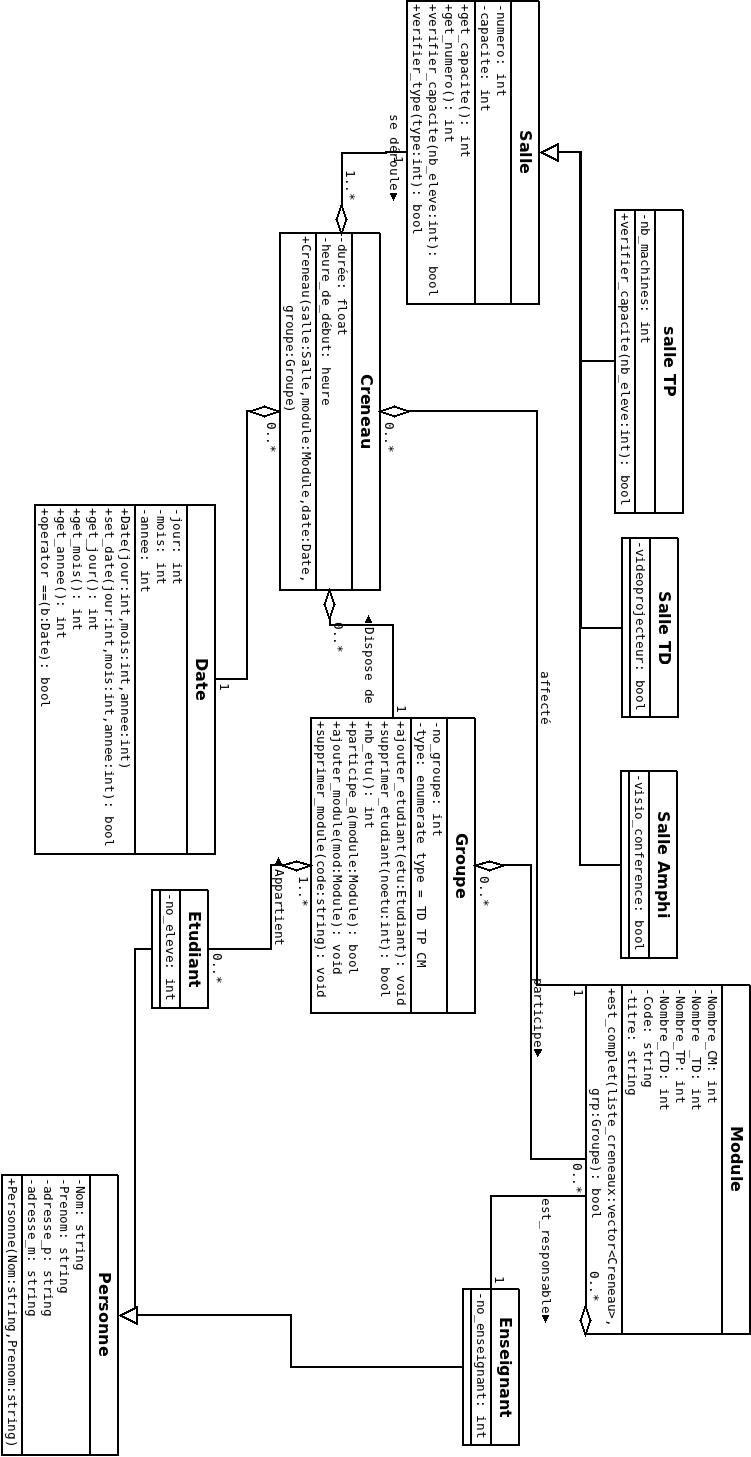
\includegraphics[height=23cm]{diagclasse}
	\end{center}
	On ajoute à ce diagramme déjà chargé quelques contraintes et spécifications :
	\begin{itemize}
	 \item Les agrégations seront implémentés sous forme de pointeur ou ensemble trié pointeurs, afin de récupérer directement la liste des objets sous forme triée.
	 \item Les paramètres des fonctions et méthodes peuvent devenir constants, pointeurs... selon les besoins de l'implémentation.
	 \item Les méthodes d'accès aux variables ne sont pas précisées dans le schéma mais devront apparaître.
	 \item L'exception à la clause ci-dessus revient aux enseignants et étudiants, dont on n'autorise pas les changement de numéro (identifiants dans notre modèle)
	\end{itemize}
	
	\section{Les Classes}
	\subsection{Personne}
		La classe personne est simple, et résume les attributs et getters / setters associés communs aux professeurs et étudiants. Ainsi, tout le monde possède un nom, un prénom, une adresse postale et une adresse de courriel.
	\subsection{Étudiant et Enseignant}
		Ces deux classes se ressemblent car elles spécialisent la classe Personne en ajoutant un numéro d'identifiant, et ses getters et setters associés. Nous aurions put implémenter un attribut ``type'' dans la classe personne et ainsi ne pas avoir deux classes identiques, mais notre choix de cohérence s'est tourné dans ce sens. On peut imaginer qu'un étudiant et un enseignant ne possèdent plus les mêmes méthodes dans une future évolution du projet.
		
		On remarque que la notion d'identifiant est forte car les opérateurs de comparaisons sont définis selon ce seul critère. Deux étudiants dans notre modèle ne peuvent avoir le même identifiant, il en est de même pour les enseignants.
	\subsection{Date}
		Le choix d'implémenter une classe Date nous permet de facilement trier ou comparer les dates. Lors du dialogue entre le contrôleur et la vue, on utilise exclusivement les identifiants ou pointeurs associés aux objets, à l'exception de la classe ``Date'', car nous avons considérés que l'objet est simple à créer et utiliser.
		Une classe Date possède donc les attributs entiers de type ``Jour'' ``Mois'' ``Année''. Un script de vérification lors de la création et modification d'une date vérifie que l'année est bisextile ou non, et déclenche une exception textuelle si le format est faux (de type \textbf{const char *}).
	\subsection{Module}
		Un module possède un Code. Contrairement aux identifiants des autres classes, ce code est représenté par une chaîne de caractères, et le classement des modules sera alphabétique. Cette classe possède également un nombre d'heures de TP, TD, CM ou CTD (correspondants aux CM+TD).
		
		En passant en paramètre un groupe (appartenant au module) et une liste de créneaux associés, la fonction \textbf{est\_complet} se charge de parcourir la liste de créneaux et de compter les heures faites (ou prévues) d'enseignement. Une fois les compteurs complets, la fonction s'assure que l'ensemble des heures programmées complète bien les conditions du créneau.
		On précise que le mode ``CTDi'' est détecté lorsque le nombre de CTD prévu est supérieur à 1. Ainsi, deux constructeurs ont étés implémentés pour répondre aux modules type CM TD ou CTD.
	\subsection{Salles}
		La classe Salle (abstraite) permet de généraliser les trois classes héritées : Amphi, TD, et TP. À l'image de la faculté, toutes les salles possèdent un identifiant (ici uniquement numéraire), et une capacité.
		La méthode de vérification de capacité est commune aux amphis et salles de TD, nous l'implémentons donc dans la classe mère. En revanche, nous la redéfinirons dans la classe Salle\_TP, en considérant que la capacité correspond au nombre de machine multipliée par 2.
		
		La méthode abstraite pure ``vérifier type'' est implémentée dans les trois classes filles, à l'image des exemples traités en cours.
	\subsection{Groupe}
		Un groupe est composé dans notre implémentation d'un numéro (identifiant), d'une liste de créneaux et d'une autre d'étudiants. Ces deux listes sont implémentés ici par des set de pointeurs, conformément au cahier des charges de la partie 1. 
		
		Les méthodes de suppression de module et étudiant effacent le pointeur associé s'il existe, mais ne fait rien dans le cas contraire.
	\subsection{Créneau}
		La classe créneau est l'élément central de notre schéma de classe. En effet, l'emploi du temps (contrôleur) est défini par un ensemble de créneaux, eux-mêmes composés d'un groupe suivant l'enseignement d'un module, dans une salle à une certaine date, à partir d'une heure de début en pendant une durée donnée.
		
		Les créneaux sont triés par date, puis heure, puis salle. Deux créneaux de même heure,date et lieu sont considérés comme identiques.
	\chapter{Le contrôleur}
		Le contrôleur permet de gérer entièrement un emplois du temps, utilise les classes définies ci-dessus, et permet au système de faire toutes les modifications nécessaires dans l'emplois du temps.
		
		Nous avons choisi d'implémenter le contrôleur comme une classe (Edt), ce qui nous permet de définir clairement les éléments accessibles ou non depuis l'extérieur, et ainsi d'obtenir un système entièrement hermétique. En effet, la vue devra utiliser exclusivement les fonctions et procédures autorisés par le contrôleur.
	\section{Les attributs}
		Un emplois du temps est formé d'une liste d'enseignants, une liste d'étudiants, une liste de créneaux, une liste de dates possibles (pour le créneau), une liste de salle, et une liste de module. On remarque au passage l'intérêt des dates, qui empêchent de placer un créneau en dehors des jours de cours officiels.
		
	\section{Les méthodes}
		Les guetteurs de ce contrôleurs retournent simplement les différentes listes sous la forme de constantes, ce qui n'autorise la vue qu'à utiliser les méthodes constantes issues des objets de ces listes. Par exemple, en parcourant la liste des étudiants, une vue pourra consulter les attributs de chaque étudiant, mais en aucun cas les modifier ou en supprimer / ajouter.
		
		Des fonctions internes de recherche d'objet ont étés définie afin d’alléger les autres codes. Ces fonctions cherchent l'objet dans les listes, et retournent un pointeur vers ce dernier. La principale utilité de ces fonctions est d'empêcher l'accès à des objets inexistants (numéro d'étudiant inconnu). En effet, en cas d'échec, elles lèvent une exception textuelle précisant la nature de l'échec.
	\section{Interactions}
		Nous avons choisi un contrôleur au maximum indépendant de la vue (ou des vues) associé(s). Ainsi, la vue ne communique avec le contrôleur uniquement par identifiants, et non par pointeur ou objet. Ce choix à été fait afin de pouvoir à l'avenir repenser entièrement le modèle et sa gestion sans pour autant changer l'interface graphique. Seule les dates sont encore exprimées sous forme d'objet.
		
		Lors de l'ajout d'un nouveau créneau, même si l'interface graphique à déjà fait cette vérification, le contrôleur ne créer le créneau que s'il ne possède aucune interférence avec les autres (deux créneaux qui se chevauchent dans la même salle). Il prend soin également de vérifier la capacité de la salle d'accueil en fonction du groupe.
		
	\part{A mettre en conclusion}
		L'implémentation actuelle n'est pas optimale. A l'observation des structures mises en place, un système se rapprochant d'une base de donnée (ici une map) aurait été plus judicieuse pour la recherche d'éléments. La volonté d'utiliser un contrôleur hermétique nous permet de combler ces lacunes sans toucher au système de vue (précisons au passage que le parcourt de map s'effectue de la même manière).
		Nous aurions aimé également implémenter un système de traitement de l'emploi du temps intelligent, permettant l'aide à la décision, en croisant l'ensemble de nos acquis de ces trois dernières années.
\end{document} 
